\documentclass[tikz]{standalone}
\begin{document}
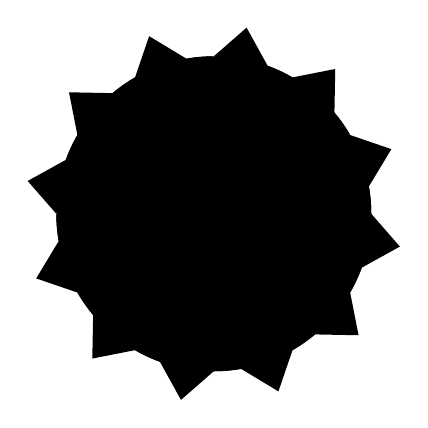
\begin{tikzpicture}

\def\teeth{12}
\def\innerR{2}
\def\outerR{2.4}
\pgfmathsetmacro\angle{360/\teeth)}

\fill (0:0) circle [radius=\innerR];
\fill
  \foreach \i in {1,2,...,\teeth} {%
     % [rotate=(\i-1)*\angle]  (0:\innerR)  arc (0:12:\innerR) -- (18:\outerR)  arc (18:30:\outerR) --  (36:\innerR)
     [rotate=(\i-1)*\angle]  (0:\innerR)  arc (0:\angle*1/3:\innerR) -- (\angle*2/3:\outerR) --  (\angle:\innerR)
   };
\end{tikzpicture} 
\end{document}